\documentclass[]{article}
\usepackage[utf8]{inputenc}
\usepackage[margin=0.5in]{geometry}
\usepackage[dvipsnames]{xcolor}
\usepackage{amsfonts, tikz, amsmath, amsthm, graphicx}

\def\docTitle{MATH261\\\large Dr. Vignon Oussa}
\def\docAuthor{Alex Dasneves}
\pagenumbering{Roman}

%Set up our counters to take over from the previous note section.
\setcounter{page}{2}
\setcounter{section}{0} %The counter for section must be 
\def\today{January 19\textsuperscript{th}, 2023}

\title{\docTitle}
\author{\docAuthor}
\date{\today}


\begin{document}
\maketitle

\section{Vectors}
\subsection{Definitions}
    \begin{enumerate}
        \item A vector is a quantity characterized by:
        \begin{enumerate}
            \item Direction
            \item Magnitude
        \end{enumerate}
        Examples:
        \begin{enumerate}
            \item Position
            \item Velocity
            \item Gravity
        \end{enumerate}
        \item A Scaler is a quantity characterized by 1 property as opposed to many\\
        Examples:
        \begin{enumerate}
            \item Mass (But not weight, as weight has a direction, caused by gravity)
            \item Speed
            \item Density
            \item Viscosity
        \end{enumerate}
        \item Standard Position: A Vector where the tail of the vector is fixed at the origin.
        \item The components of a vector are given by the coordinates of the head of the vector in standard position (\textbf{Definition 1.1.3})
        \item A unit vector is a vector of Magnitude $1$
    \end{enumerate}

    \subsection*{Geometry}
    All vectors have a head and a tail. \\
    Point A will be defined as the tail, and Point B will be defined as the head.\\
    A vector will be denoted as $v=\overrightarrow{AB}$\\

    \textbf{How can we compare 2 vectors?}\\
    2 Vectors are equal to each other if they have the have the same:
    \begin{itemize}
        \item Magnitude
        \item Direction
    \end{itemize}
    \newpage
    2 Vectors are still equal even if they are in 2 different positions.\\
    \hspace*{.2in}Magnitude is defined as the distance from the tail to the head, such that:\\
    $||v|| = \sqrt{(\Delta x)^2+(\Delta y)^2}$\\
    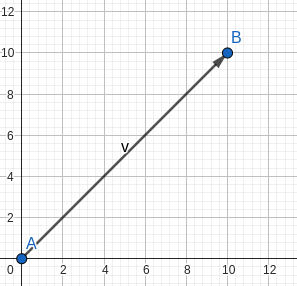
\includegraphics{Picture2.png}
    \subsection*{How to calculate Magnitude}
    If we are given a vector $\overrightarrow{AB}$, where $A=(a_1, b_1)$ and $B=(a_2, b_2)$, then $l = \sqrt{(b_2-b_1)^2+(a_2-a_1)^2}$\\
    Example:\\
        $A = (1, 2)$\\
        $B = (3, 4)$\\
        Such that:\\
        $||\overrightarrow{AB}|| = \sqrt{(3-1)^2+(4-2)^2} = \sqrt(2^2+2^2) = \sqrt{4+4} = \sqrt{2(4)} \ 2\sqrt{2}$

    If we have a 3D Vector, we can define the points as following:\\
    $A = (a_1, a_2, a_3)$\\
    $B = (b_1, b_2, b_3)$\\
    \\
    Projection onto XY Plane:\\
    $A' = (a_1, b_1, 0)$\\
    $B' = (a_2, b_2, 0)$\\
    $||\overrightarrow{A'B'}|| = \sqrt{(b_1-a_1)^2+(a_2-b_1)^2}$
    $||\overrightarrow{AB}|| = \sqrt{(b_1-a_1)^2+(b_2-a_2)^2+(b_3-a_3)^2}$

    Generalized Form for n dimensions:\\
    $||v|| = \sqrt{\Delta\dot{a}_0^2 + \Delta\dot{a}_1^2 + \cdots + \Delta\dot{a}_n^2} \Rightarrow \sqrt{(b_1 - a_1)^2 + (b_2-a_2)^2 + \cdots + (b_n-a_n)^2}$

    \subsection*{How to calculate Direction}
    %//TODO: Insert a graph with 5 vectors, with different directions and magnitudes on a 2d Cartesian Plane. 

    To get a direction, we use a unit circle.\\
    The direction of a vector is characterized by the unique vector pointing in the direction of the given vector whose tail is at the origin of space and whose head falls on the surface of a unique fixed "sphere". \\We call such a vector the unit vector. 

    %//TODO: Insert a 3d graph with a vector V, and a unit sphere about the origin. 
    Let $V = \overrightarrow{AB}$ where $A = {0, 0}$ and $B = (a_1, b_1)$\\
    The vector which starts at the tail of V, and ends on the sphere is the Unit Vector in the direction of V.

    %//TODO: Insert a graph with 2 vectors, AB, and XY, where XY is a translated AB vector, moved downwards.
    We only use Up/Down and Left/Right vectors to move a vector.

    We define a vector whose tail sits at the origin as a vector ``In Standard Position"

    Suppose we have a vector $v = \overrightarrow{AB}$ where $A = (3, 1)$ and $B = 5, 4$, as shown below:
    If we translate the vector into standard position, such that $A'$ is at $(0, 0)$, then $B'$ will be at $(2, 3)$
    We can write this vector in standard position as $v = <2,3>$
    %//TODO: Insert a graph with vector AB, with points as specified above.

    
    
    \subsection*{Geometric Vector Addition}
    To add 2 vectors, we put the tail of one vector ($\overrightarrow{AB}$) onto the tail of the other vector ($\overrightarrow{CD}$), and draw a vector, such that it is $\overrightarrow{AD}$\\

    \subsection*{Scale vectors}
    If $a > 1$, then $a \times \overrightarrow{i}$ will have a magintude greater than $i$\\
    If $0 < a < 1$, then $a \times \overrightarrow{i}$ will have a magnitude less than $i$\\
    If $a < 0$, then $a \times \overrightarrow{i}$ will have a magnitude less than $i$, but in the opposite direction\\
    if $a < -1$, then $a \times \overrightarrow{i}$ will have a magnitude greater than $i$, but in the opposite direction\\
    If $a = 0$, then $a \times \overrightarrow{i}$ will have a magnitude of 0\\

    \subsection*{Standard Basis}
    Suppose we have 2 vectors, $i = <1, 0>$ and $j = <0, 1>$\\
    We can write any vector in standard position as a combination of $(ai, bj)$\\
    For example, if we have a vector $v = <a, b>$, then $v = ai + bj$\\

    This principal also works with 3D space.\\
    We can write any vector in standard position as a combination of $(ai, bj, ck)$\\
    In 3D Space, we define the base vectors as follows:\\
    $i = <1, 0, 0>$\\
    $j = <0, 1, 0>$\\
    $k = <0, 0, 1>$\\

    Any 3D vector can be written as a linear combination of $i$, $j$, and $k$\\
    We can say that $i$, $j$, and $k$ are the standard basis vectors for 3D space.\\

    %//TODO: Insert a graph with 3 vectors, i, j, and k, and a vector v, which is a combination of i, j, and k.
    
    We can model vectors of higher dimensions as a summation of vectors.\\
    In general,\\
    \quad Of $v = <v_1, v_2, \cdots, v_n>$ and $w = <w_1, w_2, \cdots, w_n>$, then:
    \begin{equation}
        v + w = <v_1 + w_1, v_2 + w_2, \cdots, v_n + w_n>
    \end{equation}
    and
    \begin{equation}
        v-w = <v_1 - w_1, v_2 - w_2, \cdots, v_n - w_n>
    \end{equation}

    Given $\lambda \in \mathbb{R}$, we know the following:
    \begin{equation}
        \lambda v = <\lambda v_1, \lambda v_2, \cdots, \lambda v_n> \equiv <\lambda v_1, \lambda v_2, \cdots, \lambda v_n>
    \end{equation}

    Ex:\\
    \quad $v = <2, 3>$ and $w = <1, -1>$
    \begin{equation*}
        v + w = <2 + 1, 3 - 1> = <3, 2>
    \end{equation*}
    We can prove that this is correct by using the geometric method of vector addition.\\

    Say we have a vector $v = <2, 3>$, scaled by a factor of $2$. \\We can write this as $2v = 2*<2, 3> = <2 * 2, 2 * 3> = <4, 6>$\\
    
    Another Example: $v = <2, 3>$, scaled by a factor of $-2$. \\We can write this as $-2v = (-2)*<2, 3> = <-2 * 2, -2 * 3> = <-4, -6>$\\ 

    \subsection*{Unit Vector}
    Refer to the definition of a unit vector, \textbf{Definition 1.1.5}\\
    We can take the magnitude of a unit vector as follows:\\
    \begin{equation}
        \lVert \overrightarrow{v} \rVert = \sqrt{v_1^2 + v_2^2 + \cdots + v_n^2} = \sqrt{v \cdot v}
    \end{equation}
    $\lVert <1,0> \rVert$ Is a unit vector.\\
    $\lVert <0,1> \rVert$ Is a unit vector.\\
    $\lVert <2, 2> \rVert$ Is not a unit vector.\\

    How do we computer the unit vector in the direction of a given vector?\\
    \textbf{Theorem}: Let $\lambda \in \mathbb{R}$, then $\lVert \lambda v\rVert = \lvert \lambda \rvert  \lVert v \rVert$
    \textbf{Proof}: Suppose $v = <v_1, v_2, \cdots, v_n>$ where $v_i \in \mathbb{R}$, then:\\
    \begin{equation}
        \lambda v = <\lambda v_1, \lambda v_2, \cdots, \lambda v_n>
    \end{equation}\\
    \begin{equation*}
        \lVert \lambda v \rVert = \sqrt{(\lambda v_1)^2 + (\lambda v_2)^2 + \cdots + (\lambda v_n)^2}
    \end{equation*}
    $ = \sqrt{\lambda^2(v_1^2 + v_2^2 + \cdots + v_n^2)}$\\
    $ = \sqrt{\lambda^2}\sqrt{\lVert v \rVert^2}$\\
    $ = \sqrt{\lambda^2}\lVert v \rVert$\\
    $ = \lvert \lambda \rvert \lVert v \rVert$\\
    Example:
    \begin{equation*}
        \lVert -2i \rVert = 2\lVert i \rVert = 2
    \end{equation*}
    Lef $V$ be a non-zero vector\\
    let $e_v$ be the unit vector in the direction of $v$\\
    Then $e_v = \frac{v}{\lVert v \rVert}$\\
    Proof: Since $V \neq 0$, then $\lVert v \rVert \neq 0$ and $\frac{1}{\lVert v \rVert} > 0$\\
    $\frac{1}{\lVert v \rVert} \times v$ is a vector obtained by scaling v by the positive number $\frac{1}{\lVert v \rVert}$.
    $\frac{1}{\lVert v \rVert} \times v$ and $v$ have the same direction, but different magnitudes.\\
    To complete the proof, it suffices to show that $\lVert \frac{1}{\lVert v \rVert} \times v \rVert = 1$\\
    According to the previous theorum, we have:\\
    \begin{equation*}
        \lVert \frac{1}{\lVert v \rVert} \times v \rVert = \frac{1}{\lVert v \rVert} \lVert v \rVert = 1
    \end{equation*}
    This proves the proof, since multiplying $\frac{1}{x}$ by $x$ results in $1$.\\

    \paragraph*{Ex.} Given $v=<2,3>$, find $e_v$\\
    $e_v=\frac{1}{\lVert v \rVert} = \frac{1}{\sqrt{2^2+3^3}} \cdot <2,3> \frac{1}{\sqrt{13}}<2,3> = \frac{\sqrt{13}}{13}<2,3> = <\frac{2\sqrt{13}}{13}, \frac{3\sqrt{13}}{13}>$


    Suppose we have a vector in 2D space, $\overrightarrow{V}$, and we know it has an angle $\theta$.\\
    Suppose we know $\theta$, and we know $\lVert v \rVert$, can we find v?\\
    Yes, we can.\\
    \begin{equation*}
        \overrightarrow{V} = \lVert v \rVert \cdot <\cos \theta, \sin \theta> = <\lVert v \rVert \cos \theta, \lVert v \rVert \sin \theta>
    \end{equation*}
    This is the same as the conversion from polar to cartesian coordinates.\\

    Example:
    $\lVert v \rVert = 4$ and $\theta = \frac{\pi}{3} = <2, 2\sqrt{3}>$\\
    \end{document}